\documentclass[1p]{elsarticle_modified}
%\bibliographystyle{elsarticle-num}

%\usepackage[colorlinks]{hyperref}
%\usepackage{abbrmath_seonhwa} %\Abb, \Ascr, \Acal ,\Abf, \Afrak
\usepackage{amsfonts}
\usepackage{amssymb}
\usepackage{amsmath}
\usepackage{amsthm}
\usepackage{scalefnt}
\usepackage{amsbsy}
\usepackage{kotex}
\usepackage{caption}
\usepackage{subfig}
\usepackage{color}
\usepackage{graphicx}
\usepackage{xcolor} %% white, black, red, green, blue, cyan, magenta, yellow
\usepackage{float}
\usepackage{setspace}
\usepackage{hyperref}

\usepackage{tikz}
\usetikzlibrary{arrows}

\usepackage{multirow}
\usepackage{array} % fixed length table
\usepackage{hhline}

%%%%%%%%%%%%%%%%%%%%%
\makeatletter
\renewcommand*\env@matrix[1][\arraystretch]{%
	\edef\arraystretch{#1}%
	\hskip -\arraycolsep
	\let\@ifnextchar\new@ifnextchar
	\array{*\c@MaxMatrixCols c}}
\makeatother %https://tex.stackexchange.com/questions/14071/how-can-i-increase-the-line-spacing-in-a-matrix
%%%%%%%%%%%%%%%

\usepackage[normalem]{ulem}

\newcommand{\msout}[1]{\ifmmode\text{\sout{\ensuremath{#1}}}\else\sout{#1}\fi}
%SOURCE: \msout is \stkout macro in https://tex.stackexchange.com/questions/20609/strikeout-in-math-mode

\newcommand{\cancel}[1]{
	\ifmmode
	{\color{red}\msout{#1}}
	\else
	{\color{red}\sout{#1}}
	\fi
}

\newcommand{\add}[1]{
	{\color{blue}\uwave{#1}}
}

\newcommand{\replace}[2]{
	\ifmmode
	{\color{red}\msout{#1}}{\color{blue}\uwave{#2}}
	\else
	{\color{red}\sout{#1}}{\color{blue}\uwave{#2}}
	\fi
}

\newcommand{\Sol}{\mathcal{S}} %segment
\newcommand{\D}{D} %diagram
\newcommand{\A}{\mathcal{A}} %arc


%%%%%%%%%%%%%%%%%%%%%%%%%%%%%5 test

\def\sl{\operatorname{\textup{SL}}(2,\Cbb)}
\def\psl{\operatorname{\textup{PSL}}(2,\Cbb)}
\def\quan{\mkern 1mu \triangleright \mkern 1mu}

\theoremstyle{definition}
\newtheorem{thm}{Theorem}[section]
\newtheorem{prop}[thm]{Proposition}
\newtheorem{lem}[thm]{Lemma}
\newtheorem{ques}[thm]{Question}
\newtheorem{cor}[thm]{Corollary}
\newtheorem{defn}[thm]{Definition}
\newtheorem{exam}[thm]{Example}
\newtheorem{rmk}[thm]{Remark}
\newtheorem{alg}[thm]{Algorithm}

\newcommand{\I}{\sqrt{-1}}
\begin{document}

%\begin{frontmatter}
%
%\title{Boundary parabolic representations of knots up to 8 crossings}
%
%%% Group authors per affiliation:
%\author{Yunhi Cho} 
%\address{Department of Mathematics, University of Seoul, Seoul, Korea}
%\ead{yhcho@uos.ac.kr}
%
%
%\author{Seonhwa Kim} %\fnref{s_kim}}
%\address{Center for Geometry and Physics, Institute for Basic Science, Pohang, 37673, Korea}
%\ead{ryeona17@ibs.re.kr}
%
%\author{Hyuk Kim}
%\address{Department of Mathematical Sciences, Seoul National University, Seoul 08826, Korea}
%\ead{hyukkim@snu.ac.kr}
%
%\author{Seokbeom Yoon}
%\address{Department of Mathematical Sciences, Seoul National University, Seoul, 08826,  Korea}
%\ead{sbyoon15@snu.ac.kr}
%
%\begin{abstract}
%We find all boundary parabolic representation of knots up to 8 crossings.
%
%\end{abstract}
%\begin{keyword}
%    \MSC[2010] 57M25 
%\end{keyword}
%
%\end{frontmatter}

%\linenumbers
%\tableofcontents
%
\newcommand\colored[1]{\textcolor{white}{\rule[-0.35ex]{0.8em}{1.4ex}}\kern-0.8em\color{red} #1}%
%\newcommand\colored[1]{\textcolor{white}{ #1}\kern-2.17ex	\textcolor{white}{ #1}\kern-1.81ex	\textcolor{white}{ #1}\kern-2.15ex\color{red}#1	}

{\Large $\underline{12n_{0030}~(K12n_{0030})}$}

\setlength{\tabcolsep}{10pt}
\renewcommand{\arraystretch}{1.6}
\vspace{1cm}\begin{tabular}{m{100pt}>{\centering\arraybackslash}m{274pt}}
\multirow{5}{120pt}{
	\centering
	\includegraphics[width=112pt]{../../../GIT/diagram.site/Diagrams/png/2119_12n_0030.png}\\
\ \ \ A knot diagram\footnotemark}&
\allowdisplaybreaks
\textbf{Linearized knot diagam} \\
\cline{2-2}
 &
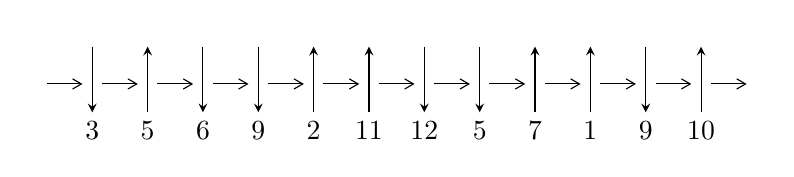
\begin{tikzpicture}[x=20pt, y=17pt]
	% nodes
	\node (C0) at (0, 0) {};
	\node (C1) at (1, 0) {};
	\node (C1U) at (1, +1) {};
	\node (C1D) at (1, -1) {3};

	\node (C2) at (2, 0) {};
	\node (C2U) at (2, +1) {};
	\node (C2D) at (2, -1) {5};

	\node (C3) at (3, 0) {};
	\node (C3U) at (3, +1) {};
	\node (C3D) at (3, -1) {6};

	\node (C4) at (4, 0) {};
	\node (C4U) at (4, +1) {};
	\node (C4D) at (4, -1) {9};

	\node (C5) at (5, 0) {};
	\node (C5U) at (5, +1) {};
	\node (C5D) at (5, -1) {2};

	\node (C6) at (6, 0) {};
	\node (C6U) at (6, +1) {};
	\node (C6D) at (6, -1) {11};

	\node (C7) at (7, 0) {};
	\node (C7U) at (7, +1) {};
	\node (C7D) at (7, -1) {12};

	\node (C8) at (8, 0) {};
	\node (C8U) at (8, +1) {};
	\node (C8D) at (8, -1) {5};

	\node (C9) at (9, 0) {};
	\node (C9U) at (9, +1) {};
	\node (C9D) at (9, -1) {7};

	\node (C10) at (10, 0) {};
	\node (C10U) at (10, +1) {};
	\node (C10D) at (10, -1) {1};

	\node (C11) at (11, 0) {};
	\node (C11U) at (11, +1) {};
	\node (C11D) at (11, -1) {9};

	\node (C12) at (12, 0) {};
	\node (C12U) at (12, +1) {};
	\node (C12D) at (12, -1) {10};
	\node (C13) at (13, 0) {};

	% arrows
	\draw[->,>={angle 60}]
	(C0) edge (C1) (C1) edge (C2) (C2) edge (C3) (C3) edge (C4) (C4) edge (C5) (C5) edge (C6) (C6) edge (C7) (C7) edge (C8) (C8) edge (C9) (C9) edge (C10) (C10) edge (C11) (C11) edge (C12) (C12) edge (C13) ;	\draw[->,>=stealth]
	(C1U) edge (C1D) (C2D) edge (C2U) (C3U) edge (C3D) (C4U) edge (C4D) (C5D) edge (C5U) (C6D) edge (C6U) (C7U) edge (C7D) (C8U) edge (C8D) (C9D) edge (C9U) (C10D) edge (C10U) (C11U) edge (C11D) (C12D) edge (C12U) ;
	\end{tikzpicture} \\
\hhline{~~} \\& 
\textbf{Solving Sequence} \\ \cline{2-2} 
 &
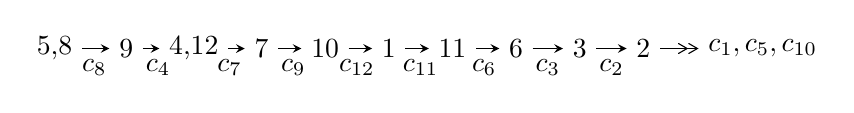
\begin{tikzpicture}[x=23pt, y=7pt]
	% node
	\node (A0) at (-1/8, 0) {5,8};
	\node (A1) at (1, 0) {9};
	\node (A2) at (33/16, 0) {4,12};
	\node (A3) at (25/8, 0) {7};
	\node (A4) at (33/8, 0) {10};
	\node (A5) at (41/8, 0) {1};
	\node (A6) at (49/8, 0) {11};
	\node (A7) at (57/8, 0) {6};
	\node (A8) at (65/8, 0) {3};
	\node (A9) at (73/8, 0) {2};
	\node (C1) at (1/2, -1) {$c_{8}$};
	\node (C2) at (3/2, -1) {$c_{4}$};
	\node (C3) at (21/8, -1) {$c_{7}$};
	\node (C4) at (29/8, -1) {$c_{9}$};
	\node (C5) at (37/8, -1) {$c_{12}$};
	\node (C6) at (45/8, -1) {$c_{11}$};
	\node (C7) at (53/8, -1) {$c_{6}$};
	\node (C8) at (61/8, -1) {$c_{3}$};
	\node (C9) at (69/8, -1) {$c_{2}$};
	\node (A10) at (11, 0) {$c_{1},c_{5},c_{10}$};

	% edge
	\draw[->,>=stealth]	
	(A0) edge (A1) (A1) edge (A2) (A2) edge (A3) (A3) edge (A4) (A4) edge (A5) (A5) edge (A6) (A6) edge (A7) (A7) edge (A8) (A8) edge (A9) ;
	\draw[->>,>={angle 60}]	
	(A9) edge (A10);
\end{tikzpicture} \\ 

\end{tabular} \\

\footnotetext{
The image of knot diagram is generated by the software ``\textbf{Draw programme}" developed by Andrew Bartholomew(\url{http://www.layer8.co.uk/maths/draw/index.htm\#Running-draw}), where we modified some parts for our purpose(\url{https://github.com/CATsTAILs/LinksPainter}).
}\phantom \\ \newline 
\centering \textbf{Ideals for irreducible components\footnotemark of $X_{\text{par}}$} 
 
\begin{align*}
I^u_{1}&=\langle 
3.62545\times10^{313} u^{83}+6.15170\times10^{313} u^{82}+\cdots+6.32484\times10^{315} b+7.92185\times10^{316},\\
\phantom{I^u_{1}}&\phantom{= \langle  }-3.59853\times10^{313} u^{83}-1.80819\times10^{314} u^{82}+\cdots+2.52993\times10^{316} a-6.87140\times10^{317},\\
\phantom{I^u_{1}}&\phantom{= \langle  }u^{84}+2 u^{83}+\cdots+3072 u+1024\rangle \\
I^u_{2}&=\langle 
2 u^3+u^2+b+5 u+1,\;-3 u^3-4 u^2+a-8 u-8,\;u^4+u^3+3 u^2+2 u+1\rangle \\
\\
I^v_{1}&=\langle 
a,\;1728 v^9-4936 v^8+9872 v^7+12908 v^6-24680 v^5-34552 v^4+91527 v^3+4936 v^2+3335 b-613,\\
\phantom{I^v_{1}}&\phantom{= \langle  }v^{10}-3 v^9+6 v^8+7 v^7-16 v^6-19 v^5+58 v^4-2 v^3-7 v^2- v+1\rangle \\
\end{align*}
\raggedright * 3 irreducible components of $\dim_{\mathbb{C}}=0$, with total 98 representations.\\
\footnotetext{All coefficients of polynomials are rational numbers. But the coefficients are sometimes approximated in decimal forms when there is not enough margin.}
\newpage
\renewcommand{\arraystretch}{1}
\centering \section*{I. $I^u_{1}= \langle 3.63\times10^{313} u^{83}+6.15\times10^{313} u^{82}+\cdots+6.32\times10^{315} b+7.92\times10^{316},\;-3.60\times10^{313} u^{83}-1.81\times10^{314} u^{82}+\cdots+2.53\times10^{316} a-6.87\times10^{317},\;u^{84}+2 u^{83}+\cdots+3072 u+1024 \rangle$}
\flushleft \textbf{(i) Arc colorings}\\
\begin{tabular}{m{7pt} m{180pt} m{7pt} m{180pt} }
\flushright $a_{5}=$&$\begin{pmatrix}0\\u\end{pmatrix}$ \\
\flushright $a_{8}=$&$\begin{pmatrix}1\\0\end{pmatrix}$ \\
\flushright $a_{9}=$&$\begin{pmatrix}1\\u^2\end{pmatrix}$ \\
\flushright $a_{4}=$&$\begin{pmatrix}u\\u^3+u\end{pmatrix}$ \\
\flushright $a_{12}=$&$\begin{pmatrix}0.00142238 u^{83}+0.00714717 u^{82}+\cdots+4.37921 u+27.1604\\-0.00573208 u^{83}-0.00972627 u^{82}+\cdots-21.7493 u-12.5250\end{pmatrix}$ \\
\flushright $a_{7}=$&$\begin{pmatrix}-0.00440220 u^{83}-0.0155721 u^{82}+\cdots-21.1672 u-21.6501\\0.00850686 u^{83}+0.0117475 u^{82}+\cdots+21.9408 u+4.77851\end{pmatrix}$ \\
\flushright $a_{10}=$&$\begin{pmatrix}-0.00557181 u^{83}-0.00516502 u^{82}+\cdots-14.6483 u+9.47061\\0.000335853 u^{83}+0.000887942 u^{82}+\cdots-1.07766 u+3.84523\end{pmatrix}$ \\
\flushright $a_{1}=$&$\begin{pmatrix}0.00764905 u^{83}+0.0136726 u^{82}+\cdots+20.6805 u+20.3223\\0.00313239 u^{83}+0.00646405 u^{82}+\cdots+8.74407 u+11.6319\end{pmatrix}$ \\
\flushright $a_{11}=$&$\begin{pmatrix}-0.000790893 u^{83}+0.00283051 u^{82}+\cdots-2.69654 u+19.0410\\-0.00542175 u^{83}-0.00957199 u^{82}+\cdots-19.8204 u-12.6375\end{pmatrix}$ \\
\flushright $a_{6}=$&$\begin{pmatrix}0.00451666 u^{83}+0.00720851 u^{82}+\cdots+11.9364 u+8.69044\\-0.00262839 u^{83}-0.00551221 u^{82}+\cdots-7.76333 u-9.76326\end{pmatrix}$ \\
\flushright $a_{3}=$&$\begin{pmatrix}-0.0106686 u^{83}-0.0158171 u^{82}+\cdots-36.1449 u-16.7400\\-0.00641780 u^{83}-0.0100395 u^{82}+\cdots-20.3360 u-13.7909\end{pmatrix}$ \\
\flushright $a_{2}=$&$\begin{pmatrix}-0.0106686 u^{83}-0.0158171 u^{82}+\cdots-36.1449 u-16.7400\\-0.00837526 u^{83}-0.0135852 u^{82}+\cdots-26.3690 u-19.4434\end{pmatrix}$\\&\end{tabular}
\flushleft \textbf{(ii) Obstruction class $= -1$}\\~\\
\flushleft \textbf{(iii) Cusp Shapes $= -0.0168619 u^{83}-0.00458246 u^{82}+\cdots+15.0455 u+47.7451$}\\~\\
\newpage\renewcommand{\arraystretch}{1}
\flushleft \textbf{(iv) u-Polynomials at the component}\newline \\
\begin{tabular}{m{50pt}|m{274pt}}
Crossings & \hspace{64pt}u-Polynomials at each crossing \\
\hline $$\begin{aligned}c_{1}\end{aligned}$$&$\begin{aligned}
&u^{84}+43 u^{83}+\cdots-18 u+1
\end{aligned}$\\
\hline $$\begin{aligned}c_{2},c_{5}\end{aligned}$$&$\begin{aligned}
&u^{84}+7 u^{83}+\cdots+8 u+1
\end{aligned}$\\
\hline $$\begin{aligned}c_{3}\end{aligned}$$&$\begin{aligned}
&u^{84}-7 u^{83}+\cdots+18564 u+47236
\end{aligned}$\\
\hline $$\begin{aligned}c_{4},c_{8}\end{aligned}$$&$\begin{aligned}
&u^{84}+2 u^{83}+\cdots+3072 u+1024
\end{aligned}$\\
\hline $$\begin{aligned}c_{6}\end{aligned}$$&$\begin{aligned}
&u^{84}-5 u^{83}+\cdots+78942 u+33589
\end{aligned}$\\
\hline $$\begin{aligned}c_{7}\end{aligned}$$&$\begin{aligned}
&u^{84}+u^{83}+\cdots-1664 u+101
\end{aligned}$\\
\hline $$\begin{aligned}c_{9}\end{aligned}$$&$\begin{aligned}
&u^{84}+4 u^{83}+\cdots+3 u+1
\end{aligned}$\\
\hline $$\begin{aligned}c_{10},c_{12}\end{aligned}$$&$\begin{aligned}
&u^{84}+7 u^{83}+\cdots+19 u+1
\end{aligned}$\\
\hline $$\begin{aligned}c_{11}\end{aligned}$$&$\begin{aligned}
&u^{84}-13 u^{83}+\cdots+104 u+16
\end{aligned}$\\
\hline
\end{tabular}\\~\\
\newpage\renewcommand{\arraystretch}{1}
\flushleft \textbf{(v) Riley Polynomials at the component}\newline \\
\begin{tabular}{m{50pt}|m{274pt}}
Crossings & \hspace{64pt}Riley Polynomials at each crossing \\
\hline $$\begin{aligned}c_{1}\end{aligned}$$&$\begin{aligned}
&y^{84}+3 y^{83}+\cdots-590 y+1
\end{aligned}$\\
\hline $$\begin{aligned}c_{2},c_{5}\end{aligned}$$&$\begin{aligned}
&y^{84}+43 y^{83}+\cdots-18 y+1
\end{aligned}$\\
\hline $$\begin{aligned}c_{3}\end{aligned}$$&$\begin{aligned}
&y^{84}-37 y^{83}+\cdots-5800852456 y+2231239696
\end{aligned}$\\
\hline $$\begin{aligned}c_{4},c_{8}\end{aligned}$$&$\begin{aligned}
&y^{84}-50 y^{83}+\cdots-22020096 y+1048576
\end{aligned}$\\
\hline $$\begin{aligned}c_{6}\end{aligned}$$&$\begin{aligned}
&y^{84}+85 y^{83}+\cdots-18778069822 y+1128220921
\end{aligned}$\\
\hline $$\begin{aligned}c_{7}\end{aligned}$$&$\begin{aligned}
&y^{84}+69 y^{83}+\cdots-1278338 y+10201
\end{aligned}$\\
\hline $$\begin{aligned}c_{9}\end{aligned}$$&$\begin{aligned}
&y^{84}-24 y^{83}+\cdots+11 y+1
\end{aligned}$\\
\hline $$\begin{aligned}c_{10},c_{12}\end{aligned}$$&$\begin{aligned}
&y^{84}-49 y^{83}+\cdots-211 y+1
\end{aligned}$\\
\hline $$\begin{aligned}c_{11}\end{aligned}$$&$\begin{aligned}
&y^{84}-21 y^{83}+\cdots-19776 y+256
\end{aligned}$\\
\hline
\end{tabular}\\~\\
\newpage\flushleft \textbf{(vi) Complex Volumes and Cusp Shapes}
$$\begin{array}{c|c|c}  
\text{Solutions to }I^u_{1}& \I (\text{vol} + \sqrt{-1}CS) & \text{Cusp shape}\\
 \hline 
\begin{aligned}
u &= -0.841987 + 0.437455 I \\
a &= -0.264125 - 1.135590 I \\
b &= -0.274994 - 0.228453 I\end{aligned}
 & -0.303408 + 1.335140 I & \phantom{-0.000000 } 0 \\ \hline\begin{aligned}
u &= -0.841987 - 0.437455 I \\
a &= -0.264125 + 1.135590 I \\
b &= -0.274994 + 0.228453 I\end{aligned}
 & -0.303408 - 1.335140 I & \phantom{-0.000000 } 0 \\ \hline\begin{aligned}
u &= \phantom{-}0.886655 + 0.055494 I \\
a &= -1.59300 + 1.49212 I \\
b &= -0.527659 + 0.467864 I\end{aligned}
 & -0.72347 + 3.79694 I & -4.78687 - 5.26590 I \\ \hline\begin{aligned}
u &= \phantom{-}0.886655 - 0.055494 I \\
a &= -1.59300 - 1.49212 I \\
b &= -0.527659 - 0.467864 I\end{aligned}
 & -0.72347 - 3.79694 I & -4.78687 + 5.26590 I \\ \hline\begin{aligned}
u &= \phantom{-}1.072820 + 0.309098 I \\
a &= \phantom{-}0.342724 - 0.766994 I \\
b &= \phantom{-}0.220027 + 1.047230 I\end{aligned}
 & \phantom{-}0.99043 - 3.63889 I & \phantom{-0.000000 } 0 \\ \hline\begin{aligned}
u &= \phantom{-}1.072820 - 0.309098 I \\
a &= \phantom{-}0.342724 + 0.766994 I \\
b &= \phantom{-}0.220027 - 1.047230 I\end{aligned}
 & \phantom{-}0.99043 + 3.63889 I & \phantom{-0.000000 } 0 \\ \hline\begin{aligned}
u &= -1.141120 + 0.127904 I \\
a &= -0.75584 + 1.46099 I \\
b &= -0.19924 + 2.65235 I\end{aligned}
 & -0.637274 + 0.732588 I & \phantom{-0.000000 } 0 \\ \hline\begin{aligned}
u &= -1.141120 - 0.127904 I \\
a &= -0.75584 - 1.46099 I \\
b &= -0.19924 - 2.65235 I\end{aligned}
 & -0.637274 - 0.732588 I & \phantom{-0.000000 } 0 \\ \hline\begin{aligned}
u &= -0.046941 + 1.155630 I \\
a &= \phantom{-}0.338929 + 0.087109 I \\
b &= \phantom{-}0.748631 + 0.426172 I\end{aligned}
 & -3.15026 - 4.66896 I & \phantom{-0.000000 } 0 \\ \hline\begin{aligned}
u &= -0.046941 - 1.155630 I \\
a &= \phantom{-}0.338929 - 0.087109 I \\
b &= \phantom{-}0.748631 - 0.426172 I\end{aligned}
 & -3.15026 + 4.66896 I & \phantom{-0.000000 } 0\\
 \hline 
 \end{array}$$\newpage$$\begin{array}{c|c|c}  
\text{Solutions to }I^u_{1}& \I (\text{vol} + \sqrt{-1}CS) & \text{Cusp shape}\\
 \hline 
\begin{aligned}
u &= -1.186540 + 0.223808 I \\
a &= \phantom{-}1.61465 + 0.24749 I \\
b &= \phantom{-}0.276148 - 0.192975 I\end{aligned}
 & -0.33247 + 3.91395 I & \phantom{-0.000000 } 0 \\ \hline\begin{aligned}
u &= -1.186540 - 0.223808 I \\
a &= \phantom{-}1.61465 - 0.24749 I \\
b &= \phantom{-}0.276148 + 0.192975 I\end{aligned}
 & -0.33247 - 3.91395 I & \phantom{-0.000000 } 0 \\ \hline\begin{aligned}
u &= \phantom{-}0.790274\phantom{ +0.000000I} \\
a &= \phantom{-}2.22730\phantom{ +0.000000I} \\
b &= -0.0927414\phantom{ +0.000000I}\end{aligned}
 & \phantom{-}2.51357\phantom{ +0.000000I} & \phantom{-}6.43370\phantom{ +0.000000I} \\ \hline\begin{aligned}
u &= \phantom{-}0.471133 + 1.126030 I \\
a &= \phantom{-}0.225686 + 0.214193 I \\
b &= \phantom{-}0.489548 + 0.020552 I\end{aligned}
 & -2.28832 + 2.96266 I & \phantom{-0.000000 } 0 \\ \hline\begin{aligned}
u &= \phantom{-}0.471133 - 1.126030 I \\
a &= \phantom{-}0.225686 - 0.214193 I \\
b &= \phantom{-}0.489548 - 0.020552 I\end{aligned}
 & -2.28832 - 2.96266 I & \phantom{-0.000000 } 0 \\ \hline\begin{aligned}
u &= -1.229850 + 0.012969 I \\
a &= \phantom{-}0.363787 + 0.498046 I \\
b &= \phantom{-}0.341018 - 1.175440 I\end{aligned}
 & -2.69617 + 0.11948 I & \phantom{-0.000000 } 0 \\ \hline\begin{aligned}
u &= -1.229850 - 0.012969 I \\
a &= \phantom{-}0.363787 - 0.498046 I \\
b &= \phantom{-}0.341018 + 1.175440 I\end{aligned}
 & -2.69617 - 0.11948 I & \phantom{-0.000000 } 0 \\ \hline\begin{aligned}
u &= -0.231724 + 0.709721 I \\
a &= \phantom{-}1.98561 + 2.84121 I \\
b &= -0.396332 - 0.930995 I\end{aligned}
 & \phantom{-}1.55672 - 3.93406 I & \phantom{-}5.95351 + 6.01840 I \\ \hline\begin{aligned}
u &= -0.231724 - 0.709721 I \\
a &= \phantom{-}1.98561 - 2.84121 I \\
b &= -0.396332 + 0.930995 I\end{aligned}
 & \phantom{-}1.55672 + 3.93406 I & \phantom{-}5.95351 - 6.01840 I \\ \hline\begin{aligned}
u &= \phantom{-}0.443646 + 0.570101 I \\
a &= \phantom{-}2.38081 - 1.64856 I \\
b &= -0.357450 + 0.659687 I\end{aligned}
 & \phantom{-}2.97676 + 0.06912 I & \phantom{-}8.15601 - 0.00886 I\\
 \hline 
 \end{array}$$\newpage$$\begin{array}{c|c|c}  
\text{Solutions to }I^u_{1}& \I (\text{vol} + \sqrt{-1}CS) & \text{Cusp shape}\\
 \hline 
\begin{aligned}
u &= \phantom{-}0.443646 - 0.570101 I \\
a &= \phantom{-}2.38081 + 1.64856 I \\
b &= -0.357450 - 0.659687 I\end{aligned}
 & \phantom{-}2.97676 - 0.06912 I & \phantom{-}8.15601 + 0.00886 I \\ \hline\begin{aligned}
u &= \phantom{-}0.535311 + 0.479375 I \\
a &= \phantom{-}0.553170 + 0.091063 I \\
b &= \phantom{-}0.530724 - 0.879230 I\end{aligned}
 & -0.20954 + 2.08673 I & -1.51899 - 3.33594 I \\ \hline\begin{aligned}
u &= \phantom{-}0.535311 - 0.479375 I \\
a &= \phantom{-}0.553170 - 0.091063 I \\
b &= \phantom{-}0.530724 + 0.879230 I\end{aligned}
 & -0.20954 - 2.08673 I & -1.51899 + 3.33594 I \\ \hline\begin{aligned}
u &= -0.446102 + 0.557829 I \\
a &= \phantom{-}0.651382 - 0.372945 I \\
b &= -0.221050 - 0.694468 I\end{aligned}
 & -0.194651 + 1.319340 I & -1.46532 - 4.00362 I \\ \hline\begin{aligned}
u &= -0.446102 - 0.557829 I \\
a &= \phantom{-}0.651382 + 0.372945 I \\
b &= -0.221050 + 0.694468 I\end{aligned}
 & -0.194651 - 1.319340 I & -1.46532 + 4.00362 I \\ \hline\begin{aligned}
u &= \phantom{-}0.597250 + 0.382933 I \\
a &= \phantom{-}0.86560 - 2.16525 I \\
b &= \phantom{-}0.402385 + 0.725463 I\end{aligned}
 & \phantom{-}2.92160 - 2.77404 I & \phantom{-}6.32422 + 8.38902 I \\ \hline\begin{aligned}
u &= \phantom{-}0.597250 - 0.382933 I \\
a &= \phantom{-}0.86560 + 2.16525 I \\
b &= \phantom{-}0.402385 - 0.725463 I\end{aligned}
 & \phantom{-}2.92160 + 2.77404 I & \phantom{-}6.32422 - 8.38902 I \\ \hline\begin{aligned}
u &= -0.100108 + 0.676504 I \\
a &= \phantom{-}2.46560 + 3.99891 I \\
b &= -0.62925 - 1.63616 I\end{aligned}
 & \phantom{-}0.83780 + 1.60534 I & \phantom{-}11.55428 - 5.80054 I \\ \hline\begin{aligned}
u &= -0.100108 - 0.676504 I \\
a &= \phantom{-}2.46560 - 3.99891 I \\
b &= -0.62925 + 1.63616 I\end{aligned}
 & \phantom{-}0.83780 - 1.60534 I & \phantom{-}11.55428 + 5.80054 I \\ \hline\begin{aligned}
u &= -0.210845 + 0.645700 I \\
a &= \phantom{-}0.524500 - 0.248408 I \\
b &= \phantom{-}0.297103 - 0.522586 I\end{aligned}
 & -0.081645 + 1.388350 I & -0.20547 - 3.77437 I\\
 \hline 
 \end{array}$$\newpage$$\begin{array}{c|c|c}  
\text{Solutions to }I^u_{1}& \I (\text{vol} + \sqrt{-1}CS) & \text{Cusp shape}\\
 \hline 
\begin{aligned}
u &= -0.210845 - 0.645700 I \\
a &= \phantom{-}0.524500 + 0.248408 I \\
b &= \phantom{-}0.297103 + 0.522586 I\end{aligned}
 & -0.081645 - 1.388350 I & -0.20547 + 3.77437 I \\ \hline\begin{aligned}
u &= -0.449648 + 0.505965 I \\
a &= \phantom{-}0.733323 - 0.546576 I \\
b &= \phantom{-}0.002097 - 0.373578 I\end{aligned}
 & -0.176677 + 1.378470 I & -2.64856 - 4.43072 I \\ \hline\begin{aligned}
u &= -0.449648 - 0.505965 I \\
a &= \phantom{-}0.733323 + 0.546576 I \\
b &= \phantom{-}0.002097 + 0.373578 I\end{aligned}
 & -0.176677 - 1.378470 I & -2.64856 + 4.43072 I \\ \hline\begin{aligned}
u &= \phantom{-}0.232207 + 1.303470 I \\
a &= \phantom{-}0.0976042 - 0.0966176 I \\
b &= -1.032530 + 0.870360 I\end{aligned}
 & \phantom{-}2.64295 + 5.32501 I & \phantom{-0.000000 } 0 \\ \hline\begin{aligned}
u &= \phantom{-}0.232207 - 1.303470 I \\
a &= \phantom{-}0.0976042 + 0.0966176 I \\
b &= -1.032530 - 0.870360 I\end{aligned}
 & \phantom{-}2.64295 - 5.32501 I & \phantom{-0.000000 } 0 \\ \hline\begin{aligned}
u &= -1.263120 + 0.405364 I \\
a &= \phantom{-}0.179173 + 0.675618 I \\
b &= \phantom{-}0.126913 - 1.133430 I\end{aligned}
 & -1.81006 + 8.25159 I & \phantom{-0.000000 } 0 \\ \hline\begin{aligned}
u &= -1.263120 - 0.405364 I \\
a &= \phantom{-}0.179173 - 0.675618 I \\
b &= \phantom{-}0.126913 + 1.133430 I\end{aligned}
 & -1.81006 - 8.25159 I & \phantom{-0.000000 } 0 \\ \hline\begin{aligned}
u &= \phantom{-}1.339460 + 0.104413 I \\
a &= -0.361683 + 1.004890 I \\
b &= -0.61375 + 2.46446 I\end{aligned}
 & -4.18720 - 3.29608 I & \phantom{-0.000000 } 0 \\ \hline\begin{aligned}
u &= \phantom{-}1.339460 - 0.104413 I \\
a &= -0.361683 - 1.004890 I \\
b &= -0.61375 - 2.46446 I\end{aligned}
 & -4.18720 + 3.29608 I & \phantom{-0.000000 } 0 \\ \hline\begin{aligned}
u &= \phantom{-}1.328400 + 0.308712 I \\
a &= \phantom{-}1.40163 + 0.29106 I \\
b &= \phantom{-}1.08954 + 0.93988 I\end{aligned}
 & \phantom{-}2.03077 - 8.41785 I & \phantom{-0.000000 } 0\\
 \hline 
 \end{array}$$\newpage$$\begin{array}{c|c|c}  
\text{Solutions to }I^u_{1}& \I (\text{vol} + \sqrt{-1}CS) & \text{Cusp shape}\\
 \hline 
\begin{aligned}
u &= \phantom{-}1.328400 - 0.308712 I \\
a &= \phantom{-}1.40163 - 0.29106 I \\
b &= \phantom{-}1.08954 - 0.93988 I\end{aligned}
 & \phantom{-}2.03077 + 8.41785 I & \phantom{-0.000000 } 0 \\ \hline\begin{aligned}
u &= -1.359410 + 0.160067 I \\
a &= \phantom{-}1.185480 - 0.430459 I \\
b &= \phantom{-}1.059200 - 0.760145 I\end{aligned}
 & \phantom{-}1.64539 + 2.41566 I & \phantom{-0.000000 } 0 \\ \hline\begin{aligned}
u &= -1.359410 - 0.160067 I \\
a &= \phantom{-}1.185480 + 0.430459 I \\
b &= \phantom{-}1.059200 + 0.760145 I\end{aligned}
 & \phantom{-}1.64539 - 2.41566 I & \phantom{-0.000000 } 0 \\ \hline\begin{aligned}
u &= \phantom{-}1.337020 + 0.298292 I \\
a &= -0.982452 - 0.930609 I \\
b &= -0.38347 - 2.94198 I\end{aligned}
 & -3.79074 - 5.18593 I & \phantom{-0.000000 } 0 \\ \hline\begin{aligned}
u &= \phantom{-}1.337020 - 0.298292 I \\
a &= -0.982452 + 0.930609 I \\
b &= -0.38347 + 2.94198 I\end{aligned}
 & -3.79074 + 5.18593 I & \phantom{-0.000000 } 0 \\ \hline\begin{aligned}
u &= -0.353810 + 0.514641 I \\
a &= -8.96206 - 5.53073 I \\
b &= -0.61059 + 3.96105 I\end{aligned}
 & \phantom{-}1.40295 + 1.45862 I & -89.698 - 115.931 I \\ \hline\begin{aligned}
u &= -0.353810 - 0.514641 I \\
a &= -8.96206 + 5.53073 I \\
b &= -0.61059 - 3.96105 I\end{aligned}
 & \phantom{-}1.40295 - 1.45862 I & -89.698 + 115.931 I \\ \hline\begin{aligned}
u &= \phantom{-}1.341220 + 0.421284 I \\
a &= -1.49100 + 0.04191 I \\
b &= -0.975466 - 0.634144 I\end{aligned}
 & -4.54665 - 5.72043 I & \phantom{-0.000000 } 0 \\ \hline\begin{aligned}
u &= \phantom{-}1.341220 - 0.421284 I \\
a &= -1.49100 - 0.04191 I \\
b &= -0.975466 + 0.634144 I\end{aligned}
 & -4.54665 + 5.72043 I & \phantom{-0.000000 } 0 \\ \hline\begin{aligned}
u &= \phantom{-}0.465396 + 0.288139 I \\
a &= \phantom{-}0.0853726 - 0.0912661 I \\
b &= -0.509528 + 1.280680 I\end{aligned}
 & \phantom{-}5.71423 + 6.06522 I & -1.77330 + 4.32385 I\\
 \hline 
 \end{array}$$\newpage$$\begin{array}{c|c|c}  
\text{Solutions to }I^u_{1}& \I (\text{vol} + \sqrt{-1}CS) & \text{Cusp shape}\\
 \hline 
\begin{aligned}
u &= \phantom{-}0.465396 - 0.288139 I \\
a &= \phantom{-}0.0853726 + 0.0912661 I \\
b &= -0.509528 - 1.280680 I\end{aligned}
 & \phantom{-}5.71423 - 6.06522 I & -1.77330 - 4.32385 I \\ \hline\begin{aligned}
u &= -0.490366 + 0.227601 I \\
a &= \phantom{-}0.0855734 - 0.0910038 I \\
b &= -0.361826 + 1.222090 I\end{aligned}
 & \phantom{-}5.61123 + 2.65441 I & -4.29638 - 9.51286 I \\ \hline\begin{aligned}
u &= -0.490366 - 0.227601 I \\
a &= \phantom{-}0.0855734 + 0.0910038 I \\
b &= -0.361826 - 1.222090 I\end{aligned}
 & \phantom{-}5.61123 - 2.65441 I & -4.29638 + 9.51286 I \\ \hline\begin{aligned}
u &= -0.40463 + 1.41385 I \\
a &= \phantom{-}0.0930273 + 0.1036470 I \\
b &= -1.20423 - 1.01593 I\end{aligned}
 & -0.55121 - 10.15270 I & \phantom{-0.000000 } 0 \\ \hline\begin{aligned}
u &= -0.40463 - 1.41385 I \\
a &= \phantom{-}0.0930273 - 0.1036470 I \\
b &= -1.20423 + 1.01593 I\end{aligned}
 & -0.55121 + 10.15270 I & \phantom{-0.000000 } 0 \\ \hline\begin{aligned}
u &= -1.27769 + 0.73843 I \\
a &= -0.689832 - 0.368710 I \\
b &= -0.510369 + 0.405135 I\end{aligned}
 & -2.21135 + 4.59052 I & \phantom{-0.000000 } 0 \\ \hline\begin{aligned}
u &= -1.27769 - 0.73843 I \\
a &= -0.689832 + 0.368710 I \\
b &= -0.510369 - 0.405135 I\end{aligned}
 & -2.21135 - 4.59052 I & \phantom{-0.000000 } 0 \\ \hline\begin{aligned}
u &= -0.08024 + 1.47776 I \\
a &= \phantom{-}0.114890 + 0.102038 I \\
b &= -1.193040 - 0.588194 I\end{aligned}
 & -1.47667 - 1.22264 I & \phantom{-0.000000 } 0 \\ \hline\begin{aligned}
u &= -0.08024 - 1.47776 I \\
a &= \phantom{-}0.114890 - 0.102038 I \\
b &= -1.193040 + 0.588194 I\end{aligned}
 & -1.47667 + 1.22264 I & \phantom{-0.000000 } 0 \\ \hline\begin{aligned}
u &= -0.431983 + 0.240711 I \\
a &= \phantom{-}3.56103 + 4.41691 I \\
b &= \phantom{-}0.741583 - 0.575469 I\end{aligned}
 & \phantom{-}2.34989 - 1.68894 I & -3.22664 - 4.70152 I\\
 \hline 
 \end{array}$$\newpage$$\begin{array}{c|c|c}  
\text{Solutions to }I^u_{1}& \I (\text{vol} + \sqrt{-1}CS) & \text{Cusp shape}\\
 \hline 
\begin{aligned}
u &= -0.431983 - 0.240711 I \\
a &= \phantom{-}3.56103 - 4.41691 I \\
b &= \phantom{-}0.741583 + 0.575469 I\end{aligned}
 & \phantom{-}2.34989 + 1.68894 I & -3.22664 + 4.70152 I \\ \hline\begin{aligned}
u &= -1.48932 + 0.27924 I \\
a &= \phantom{-}0.952437 + 0.255511 I \\
b &= \phantom{-}1.385620 - 0.031678 I\end{aligned}
 & -3.91699 + 0.49402 I & \phantom{-0.000000 } 0 \\ \hline\begin{aligned}
u &= -1.48932 - 0.27924 I \\
a &= \phantom{-}0.952437 - 0.255511 I \\
b &= \phantom{-}1.385620 + 0.031678 I\end{aligned}
 & -3.91699 - 0.49402 I & \phantom{-0.000000 } 0 \\ \hline\begin{aligned}
u &= \phantom{-}1.39972 + 0.58890 I \\
a &= -0.771211 + 0.440695 I \\
b &= -0.730765 - 0.241151 I\end{aligned}
 & -7.54628 - 1.28985 I & \phantom{-0.000000 } 0 \\ \hline\begin{aligned}
u &= \phantom{-}1.39972 - 0.58890 I \\
a &= -0.771211 - 0.440695 I \\
b &= -0.730765 + 0.241151 I\end{aligned}
 & -7.54628 + 1.28985 I & \phantom{-0.000000 } 0 \\ \hline\begin{aligned}
u &= -1.50848 + 0.24962 I \\
a &= -1.270500 + 0.118685 I \\
b &= -1.058770 + 0.479119 I\end{aligned}
 & -9.11776 + 1.81197 I & \phantom{-0.000000 } 0 \\ \hline\begin{aligned}
u &= -1.50848 - 0.24962 I \\
a &= -1.270500 - 0.118685 I \\
b &= -1.058770 - 0.479119 I\end{aligned}
 & -9.11776 - 1.81197 I & \phantom{-0.000000 } 0 \\ \hline\begin{aligned}
u &= -1.42256 + 0.56215 I \\
a &= -1.374560 - 0.199389 I \\
b &= -1.055600 + 0.714255 I\end{aligned}
 & -7.54281 + 10.87570 I & \phantom{-0.000000 } 0 \\ \hline\begin{aligned}
u &= -1.42256 - 0.56215 I \\
a &= -1.374560 + 0.199389 I \\
b &= -1.055600 - 0.714255 I\end{aligned}
 & -7.54281 - 10.87570 I & \phantom{-0.000000 } 0 \\ \hline\begin{aligned}
u &= \phantom{-}0.460345\phantom{ +0.000000I} \\
a &= \phantom{-}2.98021\phantom{ +0.000000I} \\
b &= -0.432563\phantom{ +0.000000I}\end{aligned}
 & \phantom{-}2.55442\phantom{ +0.000000I} & \phantom{-}4.59390\phantom{ +0.000000I}\\
 \hline 
 \end{array}$$\newpage$$\begin{array}{c|c|c}  
\text{Solutions to }I^u_{1}& \I (\text{vol} + \sqrt{-1}CS) & \text{Cusp shape}\\
 \hline 
\begin{aligned}
u &= \phantom{-}1.31857 + 0.81362 I \\
a &= -0.742286 + 0.349720 I \\
b &= -0.568332 - 0.538548 I\end{aligned}
 & -4.74130 - 10.12840 I & \phantom{-0.000000 } 0 \\ \hline\begin{aligned}
u &= \phantom{-}1.31857 - 0.81362 I \\
a &= -0.742286 - 0.349720 I \\
b &= -0.568332 + 0.538548 I\end{aligned}
 & -4.74130 + 10.12840 I & \phantom{-0.000000 } 0 \\ \hline\begin{aligned}
u &= \phantom{-}1.39322 + 0.68481 I \\
a &= \phantom{-}1.380420 - 0.253552 I \\
b &= \phantom{-}1.22232 + 1.28720 I\end{aligned}
 & -1.06531 - 12.31450 I & \phantom{-0.000000 } 0 \\ \hline\begin{aligned}
u &= \phantom{-}1.39322 - 0.68481 I \\
a &= \phantom{-}1.380420 + 0.253552 I \\
b &= \phantom{-}1.22232 - 1.28720 I\end{aligned}
 & -1.06531 + 12.31450 I & \phantom{-0.000000 } 0 \\ \hline\begin{aligned}
u &= \phantom{-}1.53635 + 0.47412 I \\
a &= \phantom{-}0.932224 - 0.321024 I \\
b &= \phantom{-}1.56257 + 0.23956 I\end{aligned}
 & -7.27588 - 5.64053 I & \phantom{-0.000000 } 0 \\ \hline\begin{aligned}
u &= \phantom{-}1.53635 - 0.47412 I \\
a &= \phantom{-}0.932224 + 0.321024 I \\
b &= \phantom{-}1.56257 - 0.23956 I\end{aligned}
 & -7.27588 + 5.64053 I & \phantom{-0.000000 } 0 \\ \hline\begin{aligned}
u &= -1.40379 + 0.79175 I \\
a &= \phantom{-}1.320760 + 0.367634 I \\
b &= \phantom{-}1.23754 - 1.38161 I\end{aligned}
 & -3.7955 + 17.8954 I & \phantom{-0.000000 } 0 \\ \hline\begin{aligned}
u &= -1.40379 - 0.79175 I \\
a &= \phantom{-}1.320760 - 0.367634 I \\
b &= \phantom{-}1.23754 + 1.38161 I\end{aligned}
 & -3.7955 - 17.8954 I & \phantom{-0.000000 } 0 \\ \hline\begin{aligned}
u &= -0.07827 + 1.61239 I \\
a &= \phantom{-}0.0768134 - 0.0133793 I \\
b &= -0.502088 + 0.081114 I\end{aligned}
 & \phantom{-}8.34326 + 3.21240 I & \phantom{-0.000000 } 0 \\ \hline\begin{aligned}
u &= -0.07827 - 1.61239 I \\
a &= \phantom{-}0.0768134 + 0.0133793 I \\
b &= -0.502088 - 0.081114 I\end{aligned}
 & \phantom{-}8.34326 - 3.21240 I & \phantom{-0.000000 } 0\\
 \hline 
 \end{array}$$\newpage$$\begin{array}{c|c|c}  
\text{Solutions to }I^u_{1}& \I (\text{vol} + \sqrt{-1}CS) & \text{Cusp shape}\\
 \hline 
\begin{aligned}
u &= -1.55633 + 0.59261 I \\
a &= \phantom{-}1.222390 + 0.124537 I \\
b &= \phantom{-}1.37056 - 1.18960 I\end{aligned}
 & -6.44809 + 8.61020 I & \phantom{-0.000000 } 0 \\ \hline\begin{aligned}
u &= -1.55633 - 0.59261 I \\
a &= \phantom{-}1.222390 - 0.124537 I \\
b &= \phantom{-}1.37056 + 1.18960 I\end{aligned}
 & -6.44809 - 8.61020 I & \phantom{-0.000000 } 0 \\ \hline\begin{aligned}
u &= \phantom{-}1.68119 + 0.16001 I \\
a &= \phantom{-}0.920196 - 0.227277 I \\
b &= \phantom{-}1.57545 - 0.24084 I\end{aligned}
 & -8.44334 + 3.92581 I & \phantom{-0.000000 } 0 \\ \hline\begin{aligned}
u &= \phantom{-}1.68119 - 0.16001 I \\
a &= \phantom{-}0.920196 + 0.227277 I \\
b &= \phantom{-}1.57545 + 0.24084 I\end{aligned}
 & -8.44334 - 3.92581 I & \phantom{-0.000000 } 0\\
 \hline 
 \end{array}$$\newpage\newpage\renewcommand{\arraystretch}{1}
\centering \section*{II. $I^u_{2}= \langle 2 u^3+u^2+b+5 u+1,\;-3 u^3-4 u^2+a-8 u-8,\;u^4+u^3+3 u^2+2 u+1 \rangle$}
\flushleft \textbf{(i) Arc colorings}\\
\begin{tabular}{m{7pt} m{180pt} m{7pt} m{180pt} }
\flushright $a_{5}=$&$\begin{pmatrix}0\\u\end{pmatrix}$ \\
\flushright $a_{8}=$&$\begin{pmatrix}1\\0\end{pmatrix}$ \\
\flushright $a_{9}=$&$\begin{pmatrix}1\\u^2\end{pmatrix}$ \\
\flushright $a_{4}=$&$\begin{pmatrix}u\\u^3+u\end{pmatrix}$ \\
\flushright $a_{12}=$&$\begin{pmatrix}3 u^3+4 u^2+8 u+8\\-2 u^3- u^2-5 u-1\end{pmatrix}$ \\
\flushright $a_{7}=$&$\begin{pmatrix}8 u^3+19 u-3\\3 u^3+4 u^2+8 u+8\end{pmatrix}$ \\
\flushright $a_{10}=$&$\begin{pmatrix}3 u^3+5 u^2+8 u+9\\-2 u^3-5 u-1\end{pmatrix}$ \\
\flushright $a_{1}=$&$\begin{pmatrix}- u^2-1\\- u^2\end{pmatrix}$ \\
\flushright $a_{11}=$&$\begin{pmatrix}3 u^3+4 u^2+8 u+8\\-2 u^3- u^2-5 u-1\end{pmatrix}$ \\
\flushright $a_{6}=$&$\begin{pmatrix}1\\0\end{pmatrix}$ \\
\flushright $a_{3}=$&$\begin{pmatrix}u^3+2 u\\u^3+u\end{pmatrix}$ \\
\flushright $a_{2}=$&$\begin{pmatrix}u^3+2 u\\u^3+u^2+2 u+1\end{pmatrix}$\\&\end{tabular}
\flushleft \textbf{(ii) Obstruction class $= 1$}\\~\\
\flushleft \textbf{(iii) Cusp Shapes $= 15 u^3+3 u^2+46 u+36$}\\~\\
\newpage\renewcommand{\arraystretch}{1}
\flushleft \textbf{(iv) u-Polynomials at the component}\newline \\
\begin{tabular}{m{50pt}|m{274pt}}
Crossings & \hspace{64pt}u-Polynomials at each crossing \\
\hline $$\begin{aligned}c_{1},c_{4}\end{aligned}$$&$\begin{aligned}
&u^4- u^3+3 u^2-2 u+1
\end{aligned}$\\
\hline $$\begin{aligned}c_{2}\end{aligned}$$&$\begin{aligned}
&u^4- u^3+u^2+1
\end{aligned}$\\
\hline $$\begin{aligned}c_{3}\end{aligned}$$&$\begin{aligned}
&u^4+u^3+5 u^2- u+2
\end{aligned}$\\
\hline $$\begin{aligned}c_{5}\end{aligned}$$&$\begin{aligned}
&u^4+u^3+u^2+1
\end{aligned}$\\
\hline $$\begin{aligned}c_{6},c_{7}\end{aligned}$$&$\begin{aligned}
&u^4-2 u^3+7 u^2-5 u+1
\end{aligned}$\\
\hline $$\begin{aligned}c_{8}\end{aligned}$$&$\begin{aligned}
&u^4+u^3+3 u^2+2 u+1
\end{aligned}$\\
\hline $$\begin{aligned}c_{9}\end{aligned}$$&$\begin{aligned}
&u^4-5 u^3+7 u^2-2 u+1
\end{aligned}$\\
\hline $$\begin{aligned}c_{10}\end{aligned}$$&$\begin{aligned}
&(u+1)^4
\end{aligned}$\\
\hline $$\begin{aligned}c_{11}\end{aligned}$$&$\begin{aligned}
&u^4
\end{aligned}$\\
\hline $$\begin{aligned}c_{12}\end{aligned}$$&$\begin{aligned}
&(u-1)^4
\end{aligned}$\\
\hline
\end{tabular}\\~\\
\newpage\renewcommand{\arraystretch}{1}
\flushleft \textbf{(v) Riley Polynomials at the component}\newline \\
\begin{tabular}{m{50pt}|m{274pt}}
Crossings & \hspace{64pt}Riley Polynomials at each crossing \\
\hline $$\begin{aligned}c_{1},c_{4},c_{8}\end{aligned}$$&$\begin{aligned}
&y^4+5 y^3+7 y^2+2 y+1
\end{aligned}$\\
\hline $$\begin{aligned}c_{2},c_{5}\end{aligned}$$&$\begin{aligned}
&y^4+y^3+3 y^2+2 y+1
\end{aligned}$\\
\hline $$\begin{aligned}c_{3}\end{aligned}$$&$\begin{aligned}
&y^4+9 y^3+31 y^2+19 y+4
\end{aligned}$\\
\hline $$\begin{aligned}c_{6},c_{7}\end{aligned}$$&$\begin{aligned}
&y^4+10 y^3+31 y^2-11 y+1
\end{aligned}$\\
\hline $$\begin{aligned}c_{9}\end{aligned}$$&$\begin{aligned}
&y^4-11 y^3+31 y^2+10 y+1
\end{aligned}$\\
\hline $$\begin{aligned}c_{10},c_{12}\end{aligned}$$&$\begin{aligned}
&(y-1)^4
\end{aligned}$\\
\hline $$\begin{aligned}c_{11}\end{aligned}$$&$\begin{aligned}
&y^4
\end{aligned}$\\
\hline
\end{tabular}\\~\\
\newpage\flushleft \textbf{(vi) Complex Volumes and Cusp Shapes}
$$\begin{array}{c|c|c}  
\text{Solutions to }I^u_{2}& \I (\text{vol} + \sqrt{-1}CS) & \text{Cusp shape}\\
 \hline 
\begin{aligned}
u &= -0.395123 + 0.506844 I \\
a &= \phantom{-}5.16441 + 2.77418 I \\
b &= \phantom{-}0.59074 - 2.34806 I\end{aligned}
 & \phantom{-}1.43393 + 1.41510 I & \phantom{-}21.1644 + 23.7210 I \\ \hline\begin{aligned}
u &= -0.395123 - 0.506844 I \\
a &= \phantom{-}5.16441 - 2.77418 I \\
b &= \phantom{-}0.59074 + 2.34806 I\end{aligned}
 & \phantom{-}1.43393 - 1.41510 I & \phantom{-}21.1644 - 23.7210 I \\ \hline\begin{aligned}
u &= -0.10488 + 1.55249 I \\
a &= -0.164409 + 0.045467 I \\
b &= \phantom{-}0.409261 - 0.055548 I\end{aligned}
 & \phantom{-}8.43568 + 3.16396 I & \phantom{-}35.3356 + 15.0782 I \\ \hline\begin{aligned}
u &= -0.10488 - 1.55249 I \\
a &= -0.164409 - 0.045467 I \\
b &= \phantom{-}0.409261 + 0.055548 I\end{aligned}
 & \phantom{-}8.43568 - 3.16396 I & \phantom{-}35.3356 - 15.0782 I\\
 \hline 
 \end{array}$$\newpage\newpage\renewcommand{\arraystretch}{1}
\centering \section*{III. $I^v_{1}= \langle a,\;1728 v^9-4936 v^8+\cdots+3335 b-613,\;v^{10}-3 v^9+\cdots- v+1 \rangle$}
\flushleft \textbf{(i) Arc colorings}\\
\begin{tabular}{m{7pt} m{180pt} m{7pt} m{180pt} }
\flushright $a_{5}=$&$\begin{pmatrix}v\\0\end{pmatrix}$ \\
\flushright $a_{8}=$&$\begin{pmatrix}1\\0\end{pmatrix}$ \\
\flushright $a_{9}=$&$\begin{pmatrix}1\\0\end{pmatrix}$ \\
\flushright $a_{4}=$&$\begin{pmatrix}v\\0\end{pmatrix}$ \\
\flushright $a_{12}=$&$\begin{pmatrix}0\\-0.518141 v^{9}+1.48006 v^{8}+\cdots-1.48006 v^{2}+0.183808\end{pmatrix}$ \\
\flushright $a_{7}=$&$\begin{pmatrix}1\\-0.462969 v^{9}+1.33373 v^{8}+\cdots-1.33373 v^{2}+1.81379\end{pmatrix}$ \\
\flushright $a_{10}=$&$\begin{pmatrix}0.462969 v^{9}-1.33373 v^{8}+\cdots+1.33373 v^{2}-0.813793\\1.14783 v^{9}-3.29565 v^{8}+\cdots+3.29565 v^{2}-1.75652\end{pmatrix}$ \\
\flushright $a_{1}=$&$\begin{pmatrix}0.684858 v^{9}-1.96192 v^{8}+\cdots+1.96192 v^{2}-0.942729\\1.14783 v^{9}-3.29565 v^{8}+\cdots+3.29565 v^{2}-1.75652\end{pmatrix}$ \\
\flushright $a_{11}=$&$\begin{pmatrix}-0.518141 v^{9}+1.48006 v^{8}+\cdots-1.48006 v^{2}+0.183808\\-0.518141 v^{9}+1.48006 v^{8}+\cdots-1.48006 v^{2}+0.183808\end{pmatrix}$ \\
\flushright $a_{6}=$&$\begin{pmatrix}-0.684858 v^{9}+1.96192 v^{8}+\cdots-1.96192 v^{2}+0.942729\\-1.14783 v^{9}+3.29565 v^{8}+\cdots-3.29565 v^{2}+1.75652\end{pmatrix}$ \\
\flushright $a_{3}=$&$\begin{pmatrix}0.0737631 v^{9}-0.147526 v^{8}+\cdots+5.22189 v-0.331634\\0.147826 v^{9}-0.295652 v^{8}+\cdots+7 v-0.756522\end{pmatrix}$ \\
\flushright $a_{2}=$&$\begin{pmatrix}-0.0740630 v^{9}+0.278561 v^{8}+\cdots+5.22189 v-0.183808\\0.147826 v^{9}-0.295652 v^{8}+\cdots+7 v-0.756522\end{pmatrix}$\\&\end{tabular}
\flushleft \textbf{(ii) Obstruction class $= 1$}\\~\\
\flushleft \textbf{(iii) Cusp Shapes $= -\frac{75}{667} v^9-\frac{30}{29} v^8+\frac{2395}{667} v^7-\frac{6267}{667} v^6-\frac{4697}{667} v^5+\frac{16833}{667} v^4+\frac{537}{29} v^3-\frac{55309}{667} v^2+\frac{263}{23} v+\frac{8994}{667}$}\\~\\
\newpage\renewcommand{\arraystretch}{1}
\flushleft \textbf{(iv) u-Polynomials at the component}\newline \\
\begin{tabular}{m{50pt}|m{274pt}}
Crossings & \hspace{64pt}u-Polynomials at each crossing \\
\hline $$\begin{aligned}c_{1},c_{3},c_{5}\end{aligned}$$&$\begin{aligned}
&(u^2- u+1)^5
\end{aligned}$\\
\hline $$\begin{aligned}c_{2}\end{aligned}$$&$\begin{aligned}
&(u^2+u+1)^5
\end{aligned}$\\
\hline $$\begin{aligned}c_{4},c_{8}\end{aligned}$$&$\begin{aligned}
&u^{10}
\end{aligned}$\\
\hline $$\begin{aligned}c_{6},c_{10}\end{aligned}$$&$\begin{aligned}
&(u^5- u^4-2 u^3+u^2+u+1)^2
\end{aligned}$\\
\hline $$\begin{aligned}c_{7}\end{aligned}$$&$\begin{aligned}
&(u^5+u^4+2 u^3+u^2+u+1)^2
\end{aligned}$\\
\hline $$\begin{aligned}c_{9}\end{aligned}$$&$\begin{aligned}
&(u^5-3 u^4+4 u^3- u^2- u+1)^2
\end{aligned}$\\
\hline $$\begin{aligned}c_{11}\end{aligned}$$&$\begin{aligned}
&(u^5- u^4+2 u^3- u^2+u-1)^2
\end{aligned}$\\
\hline $$\begin{aligned}c_{12}\end{aligned}$$&$\begin{aligned}
&(u^5+u^4-2 u^3- u^2+u-1)^2
\end{aligned}$\\
\hline
\end{tabular}\\~\\
\newpage\renewcommand{\arraystretch}{1}
\flushleft \textbf{(v) Riley Polynomials at the component}\newline \\
\begin{tabular}{m{50pt}|m{274pt}}
Crossings & \hspace{64pt}Riley Polynomials at each crossing \\
\hline $$\begin{aligned}c_{1},c_{2},c_{3}\\c_{5}\end{aligned}$$&$\begin{aligned}
&(y^2+y+1)^5
\end{aligned}$\\
\hline $$\begin{aligned}c_{4},c_{8}\end{aligned}$$&$\begin{aligned}
&y^{10}
\end{aligned}$\\
\hline $$\begin{aligned}c_{6},c_{10},c_{12}\end{aligned}$$&$\begin{aligned}
&(y^5-5 y^4+8 y^3-3 y^2- y-1)^2
\end{aligned}$\\
\hline $$\begin{aligned}c_{7},c_{11}\end{aligned}$$&$\begin{aligned}
&(y^5+3 y^4+4 y^3+y^2- y-1)^2
\end{aligned}$\\
\hline $$\begin{aligned}c_{9}\end{aligned}$$&$\begin{aligned}
&(y^5- y^4+8 y^3-3 y^2+3 y-1)^2
\end{aligned}$\\
\hline
\end{tabular}\\~\\
\newpage\flushleft \textbf{(vi) Complex Volumes and Cusp Shapes}
$$\begin{array}{c|c|c}  
\text{Solutions to }I^v_{1}& \I (\text{vol} + \sqrt{-1}CS) & \text{Cusp shape}\\
 \hline 
\begin{aligned}
v &= \phantom{-}1.38814 + 0.78973 I \\
a &= \phantom{-0.000000 } 0 \\
b &= \phantom{-}0.339110 + 0.822375 I\end{aligned}
 & \phantom{-}0.329100 + 0.499304 I & \phantom{-}2.01870 + 2.82203 I \\ \hline\begin{aligned}
v &= \phantom{-}1.38814 - 0.78973 I \\
a &= \phantom{-0.000000 } 0 \\
b &= \phantom{-}0.339110 - 0.822375 I\end{aligned}
 & \phantom{-}0.329100 - 0.499304 I & \phantom{-}2.01870 - 2.82203 I \\ \hline\begin{aligned}
v &= -1.37799 + 0.80730 I \\
a &= \phantom{-0.000000 } 0 \\
b &= \phantom{-}0.339110 + 0.822375 I\end{aligned}
 & \phantom{-}0.32910 - 3.56046 I & \phantom{-}1.95395 + 6.01185 I \\ \hline\begin{aligned}
v &= -1.37799 - 0.80730 I \\
a &= \phantom{-0.000000 } 0 \\
b &= \phantom{-}0.339110 - 0.822375 I\end{aligned}
 & \phantom{-}0.32910 + 3.56046 I & \phantom{-}1.95395 - 6.01185 I \\ \hline\begin{aligned}
v &= -0.294694 + 0.220725 I \\
a &= \phantom{-0.000000 } 0 \\
b &= -0.455697 - 1.200150 I\end{aligned}
 & \phantom{-}5.87256 - 6.43072 I & \phantom{-}6.8570 + 13.9114 I \\ \hline\begin{aligned}
v &= -0.294694 - 0.220725 I \\
a &= \phantom{-0.000000 } 0 \\
b &= -0.455697 + 1.200150 I\end{aligned}
 & \phantom{-}5.87256 + 6.43072 I & \phantom{-}6.8570 - 13.9114 I \\ \hline\begin{aligned}
v &= \phantom{-}0.338500 + 0.144851 I \\
a &= \phantom{-0.000000 } 0 \\
b &= -0.455697 - 1.200150 I\end{aligned}
 & \phantom{-}5.87256 - 2.37095 I & \phantom{-}9.93110 - 5.20350 I \\ \hline\begin{aligned}
v &= \phantom{-}0.338500 - 0.144851 I \\
a &= \phantom{-0.000000 } 0 \\
b &= -0.455697 + 1.200150 I\end{aligned}
 & \phantom{-}5.87256 + 2.37095 I & \phantom{-}9.93110 + 5.20350 I \\ \hline\begin{aligned}
v &= \phantom{-}1.44605 + 2.50463 I \\
a &= \phantom{-0.000000 } 0 \\
b &= -0.766826\phantom{ +0.000000I}\end{aligned}
 & \phantom{-}2.40108 - 2.02988 I & -2.76075 + 10.60420 I \\ \hline\begin{aligned}
v &= \phantom{-}1.44605 - 2.50463 I \\
a &= \phantom{-0.000000 } 0 \\
b &= -0.766826\phantom{ +0.000000I}\end{aligned}
 & \phantom{-}2.40108 + 2.02988 I & -2.76075 - 10.60420 I\\
 \hline 
 \end{array}$$\newpage
\newpage\renewcommand{\arraystretch}{1}
\centering \section*{ IV. u-Polynomials}
\begin{tabular}{m{50pt}|m{274pt}}
Crossings & \hspace{64pt}u-Polynomials at each crossing \\
\hline $$\begin{aligned}c_{1}\end{aligned}$$&$\begin{aligned}
&((u^2- u+1)^5)(u^4- u^3+3 u^2-2 u+1)(u^{84}+43 u^{83}+\cdots-18 u+1)
\end{aligned}$\\
\hline $$\begin{aligned}c_{2}\end{aligned}$$&$\begin{aligned}
&((u^2+u+1)^5)(u^4- u^3+u^2+1)(u^{84}+7 u^{83}+\cdots+8 u+1)
\end{aligned}$\\
\hline $$\begin{aligned}c_{3}\end{aligned}$$&$\begin{aligned}
&(u^2- u+1)^5(u^4+u^3+5 u^2- u+2)\\
&\cdot(u^{84}-7 u^{83}+\cdots+18564 u+47236)
\end{aligned}$\\
\hline $$\begin{aligned}c_{4}\end{aligned}$$&$\begin{aligned}
&u^{10}(u^4- u^3+3 u^2-2 u+1)(u^{84}+2 u^{83}+\cdots+3072 u+1024)
\end{aligned}$\\
\hline $$\begin{aligned}c_{5}\end{aligned}$$&$\begin{aligned}
&((u^2- u+1)^5)(u^4+u^3+u^2+1)(u^{84}+7 u^{83}+\cdots+8 u+1)
\end{aligned}$\\
\hline $$\begin{aligned}c_{6}\end{aligned}$$&$\begin{aligned}
&(u^4-2 u^3+7 u^2-5 u+1)(u^5- u^4-2 u^3+u^2+u+1)^2\\
&\cdot(u^{84}-5 u^{83}+\cdots+78942 u+33589)
\end{aligned}$\\
\hline $$\begin{aligned}c_{7}\end{aligned}$$&$\begin{aligned}
&(u^4-2 u^3+7 u^2-5 u+1)(u^5+u^4+2 u^3+u^2+u+1)^2\\
&\cdot(u^{84}+u^{83}+\cdots-1664 u+101)
\end{aligned}$\\
\hline $$\begin{aligned}c_{8}\end{aligned}$$&$\begin{aligned}
&u^{10}(u^4+u^3+3 u^2+2 u+1)(u^{84}+2 u^{83}+\cdots+3072 u+1024)
\end{aligned}$\\
\hline $$\begin{aligned}c_{9}\end{aligned}$$&$\begin{aligned}
&(u^4-5 u^3+7 u^2-2 u+1)(u^5-3 u^4+4 u^3- u^2- u+1)^2\\
&\cdot(u^{84}+4 u^{83}+\cdots+3 u+1)
\end{aligned}$\\
\hline $$\begin{aligned}c_{10}\end{aligned}$$&$\begin{aligned}
&((u+1)^4)(u^5- u^4+\cdots+u+1)^{2}(u^{84}+7 u^{83}+\cdots+19 u+1)
\end{aligned}$\\
\hline $$\begin{aligned}c_{11}\end{aligned}$$&$\begin{aligned}
&u^4(u^5- u^4+\cdots+u-1)^{2}(u^{84}-13 u^{83}+\cdots+104 u+16)
\end{aligned}$\\
\hline $$\begin{aligned}c_{12}\end{aligned}$$&$\begin{aligned}
&((u-1)^4)(u^5+u^4+\cdots+u-1)^{2}(u^{84}+7 u^{83}+\cdots+19 u+1)
\end{aligned}$\\
\hline
\end{tabular}\newpage\renewcommand{\arraystretch}{1}
\centering \section*{ V. Riley Polynomials}
\begin{tabular}{m{50pt}|m{274pt}}
Crossings & \hspace{64pt}Riley Polynomials at each crossing \\
\hline $$\begin{aligned}c_{1}\end{aligned}$$&$\begin{aligned}
&((y^2+y+1)^5)(y^4+5 y^3+\cdots+2 y+1)(y^{84}+3 y^{83}+\cdots-590 y+1)
\end{aligned}$\\
\hline $$\begin{aligned}c_{2},c_{5}\end{aligned}$$&$\begin{aligned}
&((y^2+y+1)^5)(y^4+y^3+3 y^2+2 y+1)(y^{84}+43 y^{83}+\cdots-18 y+1)
\end{aligned}$\\
\hline $$\begin{aligned}c_{3}\end{aligned}$$&$\begin{aligned}
&(y^2+y+1)^5(y^4+9 y^3+31 y^2+19 y+4)\\
&\cdot(y^{84}-37 y^{83}+\cdots-5800852456 y+2231239696)
\end{aligned}$\\
\hline $$\begin{aligned}c_{4},c_{8}\end{aligned}$$&$\begin{aligned}
&y^{10}(y^4+5 y^3+7 y^2+2 y+1)\\
&\cdot(y^{84}-50 y^{83}+\cdots-22020096 y+1048576)
\end{aligned}$\\
\hline $$\begin{aligned}c_{6}\end{aligned}$$&$\begin{aligned}
&(y^4+10 y^3+31 y^2-11 y+1)(y^5-5 y^4+8 y^3-3 y^2- y-1)^2\\
&\cdot(y^{84}+85 y^{83}+\cdots-18778069822 y+1128220921)
\end{aligned}$\\
\hline $$\begin{aligned}c_{7}\end{aligned}$$&$\begin{aligned}
&(y^4+10 y^3+31 y^2-11 y+1)(y^5+3 y^4+4 y^3+y^2- y-1)^2\\
&\cdot(y^{84}+69 y^{83}+\cdots-1278338 y+10201)
\end{aligned}$\\
\hline $$\begin{aligned}c_{9}\end{aligned}$$&$\begin{aligned}
&(y^4-11 y^3+31 y^2+10 y+1)(y^5- y^4+8 y^3-3 y^2+3 y-1)^2\\
&\cdot(y^{84}-24 y^{83}+\cdots+11 y+1)
\end{aligned}$\\
\hline $$\begin{aligned}c_{10},c_{12}\end{aligned}$$&$\begin{aligned}
&(y-1)^4(y^5-5 y^4+8 y^3-3 y^2- y-1)^2\\
&\cdot(y^{84}-49 y^{83}+\cdots-211 y+1)
\end{aligned}$\\
\hline $$\begin{aligned}c_{11}\end{aligned}$$&$\begin{aligned}
&y^4(y^5+3 y^4+\cdots- y-1)^{2}(y^{84}-21 y^{83}+\cdots-19776 y+256)
\end{aligned}$\\
\hline
\end{tabular}
\vskip 2pc
\end{document}